\documentclass[a4paper, 12pt, dvipdfmx]{jsarticle}  

\usepackage{geometry}
\usepackage[dvipdfmx]{graphicx}
\usepackage{booktabs}
\usepackage[dvipdfmx]{color}
\usepackage{amsmath,amssymb}
\usepackage{url}
\usepackage{listings,jlisting}
\usepackage{here}
\usepackage[dvipdfmx]{hyperref}


\usepackage{ascmac}
\usepackage{fancybx}

\geometry{
  left=15mm,
  top=15mm,
  right=15mm,
  bottom=15mm
 }


%  ソースコード表示に関する設定
 \lstset{
  basicstyle={\ttfamily},
  identifierstyle={\small},
  commentstyle={\smallitshape},
  keywordstyle={\small\bfseries},
  ndkeywordstyle={\small},
  stringstyle={\small\ttfamily},
  frame={tb},
  breaklines=true,
  columns=[l]{fullflexible},
  numbers=left,
  xrightmargin=0zw,
  xleftmargin=3zw,
  numberstyle={\scriptsize},
  stepnumber=1,
  numbersep=1zw,
  lineskip=-0.5ex
}

%
\renewcommand{\lstlistingname}{コード}
%

\title{hello}
\author{yanagihara}
\date{}

%
\begin{document}

\maketitle

\section{Introduction}\label{section:intro}

%% テンプレートです。
hoge\cite{bib:HELMHOLTZ_FURUSHO_EN}

\begin{figure}[tbp]   
  \centering   
  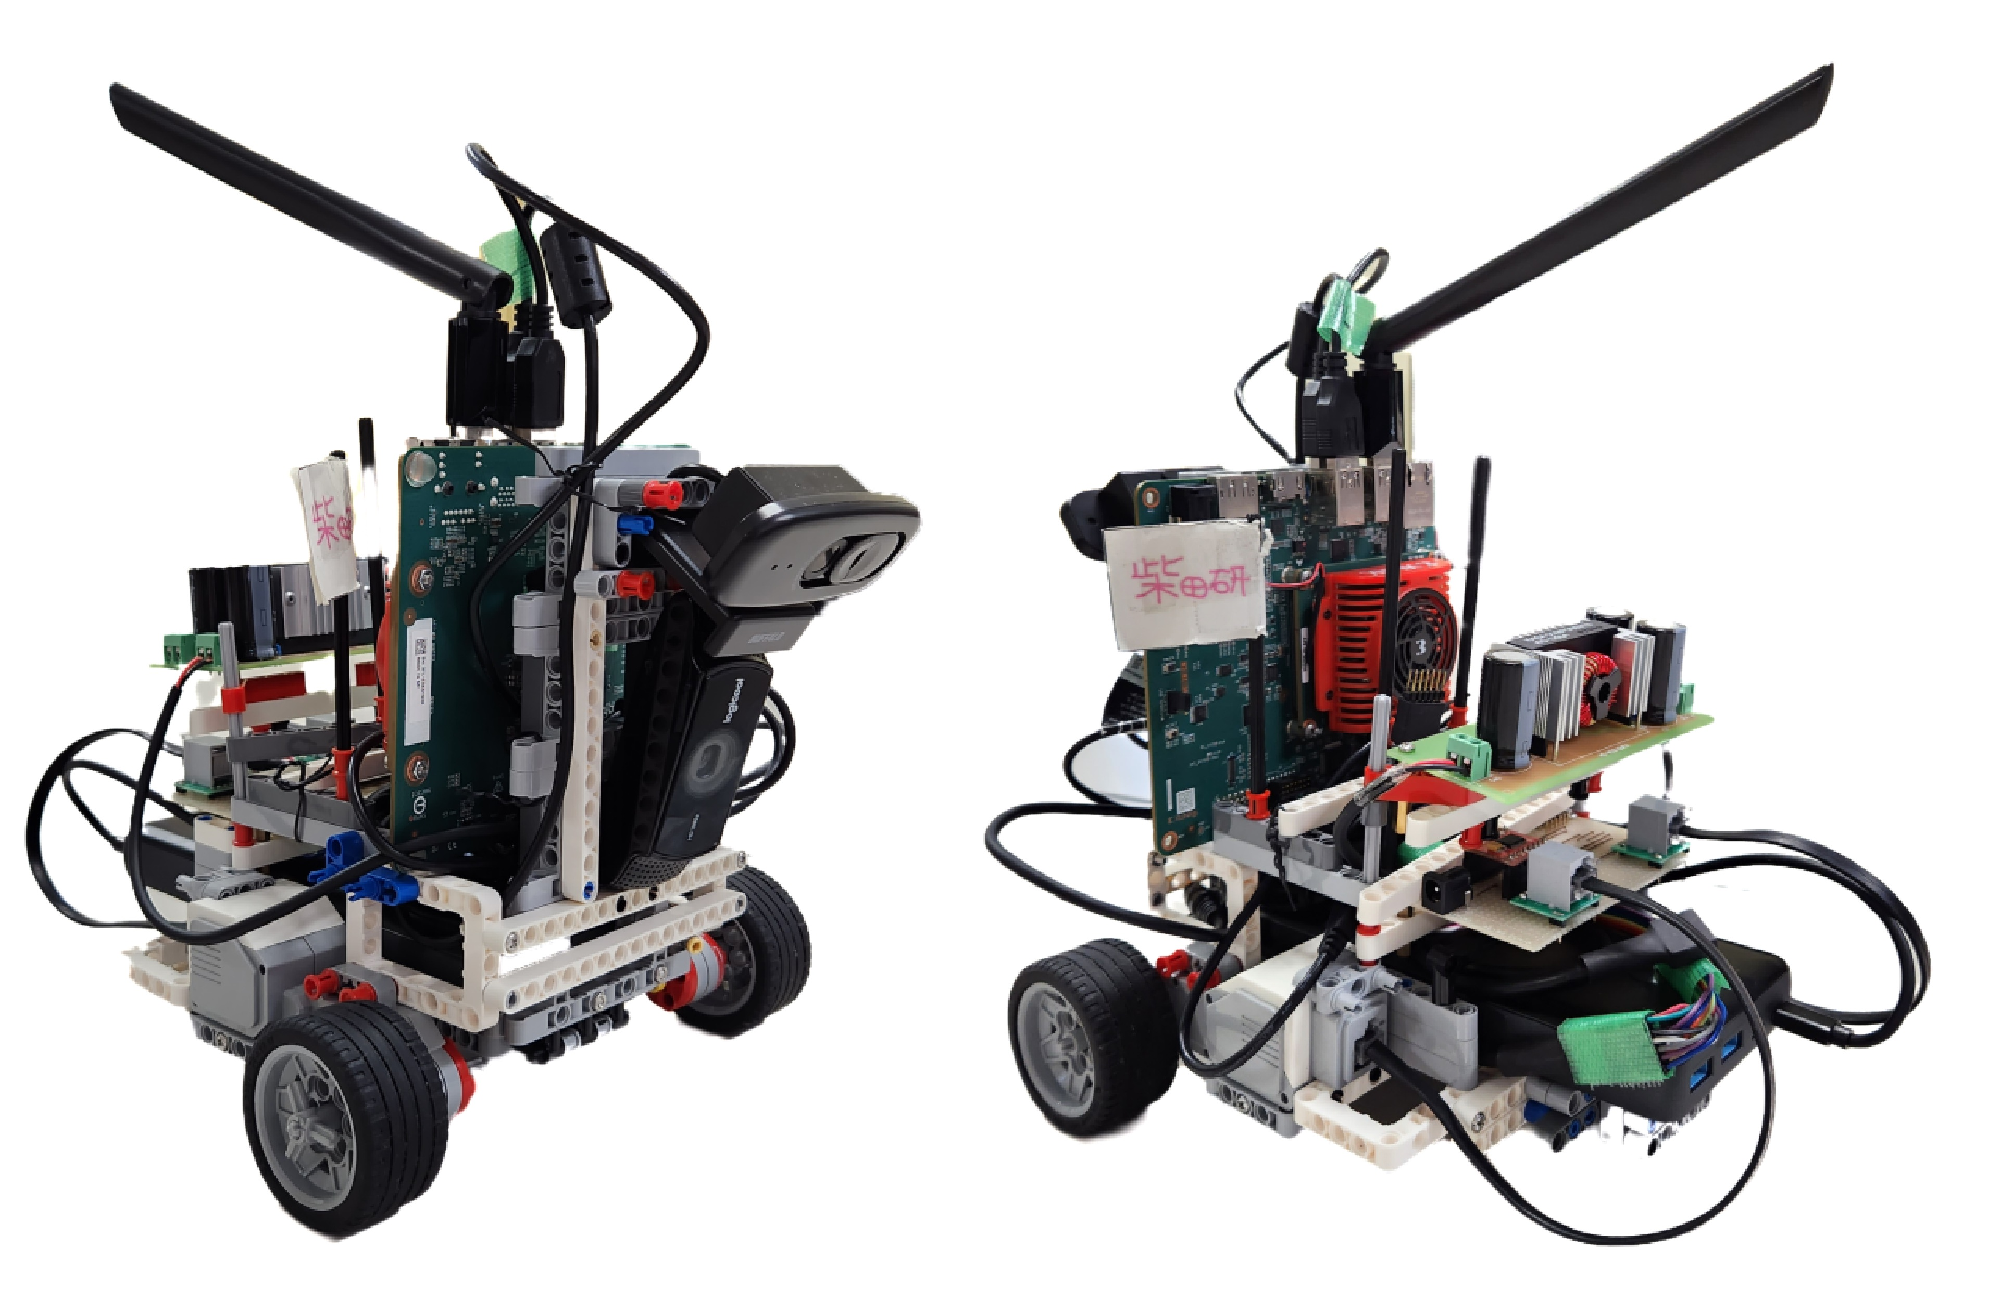
\includegraphics[width=0.48\textwidth]{img/template.pdf}
  \caption{overview}
  \label{fig:template}
\end{figure}                                                                                                             
                 



\bibliographystyle{jplain}
\bibliography{bib/0-refs.bib} 

\end{document}
%
